The histogram showed a right-skewed distribution.
Most emails are short (under 500 words), but a long tail indicates the presence of very long outlier emails, adding diversity to the dataset structure.
Length could be a potential feature.

This code calculates how many words are in each email and then creates a bar chart (histogram) to show how many emails fall into different length categories (e.g., 0–500 words, 500–1000 words, etc.). It helps visualize the typical length of emails in our dataset.

\begin{figure}[H]
    \centering
    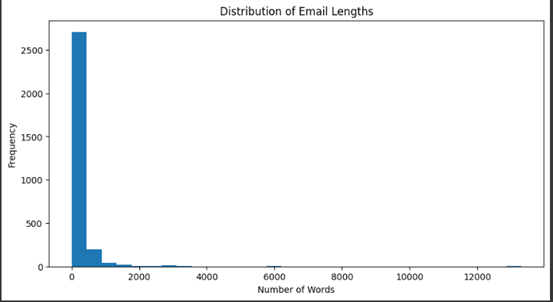
\includegraphics[width=\linewidth]{images/email_length_distribution}
    \caption{Bar Chart for Email Length Distribution}
    \label{fig:email_length_distribution}
\end{figure}

Distribution Shape:
\begin{itemize}
    \item Right-skewed: The majority of the bars are concentrated on the left side of the histogram, indicating that most emails are short in length.
    \item High Peak on the Left: The first bar (near zero words) has a significantly higher height than the other bars,showing a large number of very short emails.
    \item Long Tail to the Right: The bars gradually decrease towards the right, but there are still some emails with considerable length, extending to several thousand words.
\end{itemize}

